\documentclass[aspectratio=1610,t]{beamer}

% Tikz
\usepackage{tikz}
\usetikzlibrary{fadings}
% Colors
\usepackage{color}
\definecolor{mainorange}{HTML}{EC811B}
\definecolor{lightgrey}{HTML}{888888}

\colorlet{control}{red!20!}
\colorlet{safe}{blue!20!}
\colorlet{ok}{green!25!}

% Syntax highlighting
\usepackage{minted}
\usepackage{alltt}
\newcommand\hi[1]{{\color{mainorange} \textbf{#1}}}

% Theme
\usetheme[%
  subsectionpage=progressbar,
  numbering=fraction,
  progressbar=foot,
]{metropolis}

% Customization
\setbeamertemplate{section in toc}[sections numbered]
\setbeamerfont{title}{size=\fontsize{30}{30}}
\setbeamerfont{block title}{size=\large}
\newcommand\sep{\textcolor{lightgrey}{\rule{\linewidth}{0.05mm}}}

% Meta
\title{Rust in 5 minutes}
\date{December 30, 2016}
\author{Raphael Nestler (@rnestler)}
\institute{Coredump Hackerspace Rapperswil, Switzerland}

\begin{document}

\pgfdeclareimage[width=\paperwidth]{bg}{background-dark.pdf}
\usebackgroundtemplate{\pgfuseimage{bg}}
\maketitle

% ----------------------------------------------------------------- %

\pgfdeclareimage[width=\paperwidth]{bg}{background-light.pdf}
\usebackgroundtemplate{\pgfuseimage{bg}}

\section{What is Rust?}

\begin{frame}[c]{What is Rust?}
  \begin{columns}[onlytextwidth]
    \begin{column}{.8\textwidth}
      \begin{quote}
        «Rust is a systems programming language\\
        that runs blazingly fast, prevents nearly all segfaults,\\
        and guarantees thread safety.»\\
        \vspace{0.5em}
        {\normalfont \small --- \url{www.rust-lang.org}}
      \end{quote}
    \end{column}
    \begin{column}{.2\textwidth}
      
\includegraphics[width=\textwidth]{./rust-logo-512x512.png}
    \end{column}
  \end{columns}
\end{frame}

\begin{frame}{Control vs Safety?}
  \begin{center}
    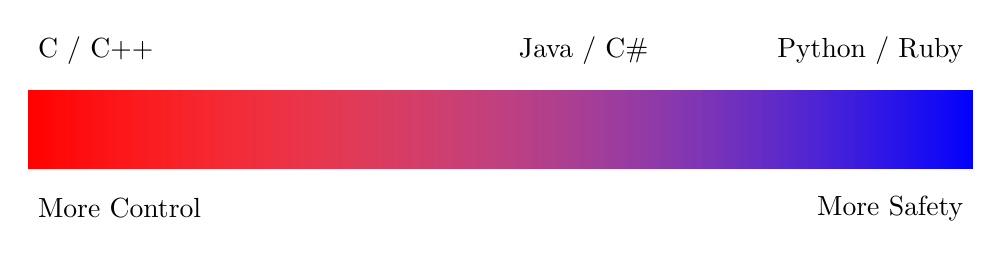
\begin{tikzpicture}
      \fill[blue,path fading=west] (-10:0) rectangle (12,1);
      \fill[red,path fading=east] (-10:0) rectangle (12,1);

      \draw (0,1.5)node[right] {C / C++} ;
      \draw (0,-0.5)node[right] {More Control} ;

      \draw (12,1.5)node[left] {Python / Ruby} ;
      \draw (8,1.5)node[left] {Java / C\#} ;
      \draw (12,-0.5)node[left] {More Safety} ;
    \end{tikzpicture}
    \pause\only<2>{\begin{figure}
\includegraphics[width=0.3\textwidth]{./why_not_both.jpg}\end{figure}}
    \only<1,3->{\begin{figure}\end{figure}}
    \pause
    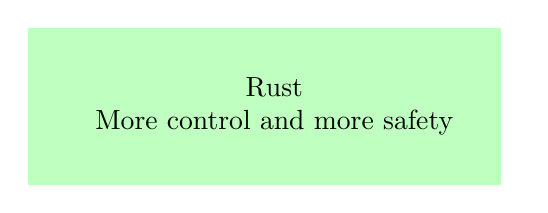
\begin{tikzpicture}
      \fill[ok] (-6:0) rectangle (6,2);
      \draw (0,1)node[right,text width=6cm,align=center]{Rust\\More control and more safety} ;
    \end{tikzpicture}

    \pause \huge{Fast, safe, concurrent, pick three!}
  \end{center}
\end{frame}

%%%

\begin{frame}[c]{A System Programming Language}
  \begin{columns}[onlytextwidth]
    \begin{column}{.4\textwidth}
      \begin{itemize}
        \item Fine grained control over memory
        \item Close to bare metal
        \item It's possible to write an OS kernel with it
      \end{itemize}
    \end{column}
    \begin{column}{.6\textwidth}
      \begin{figure}
        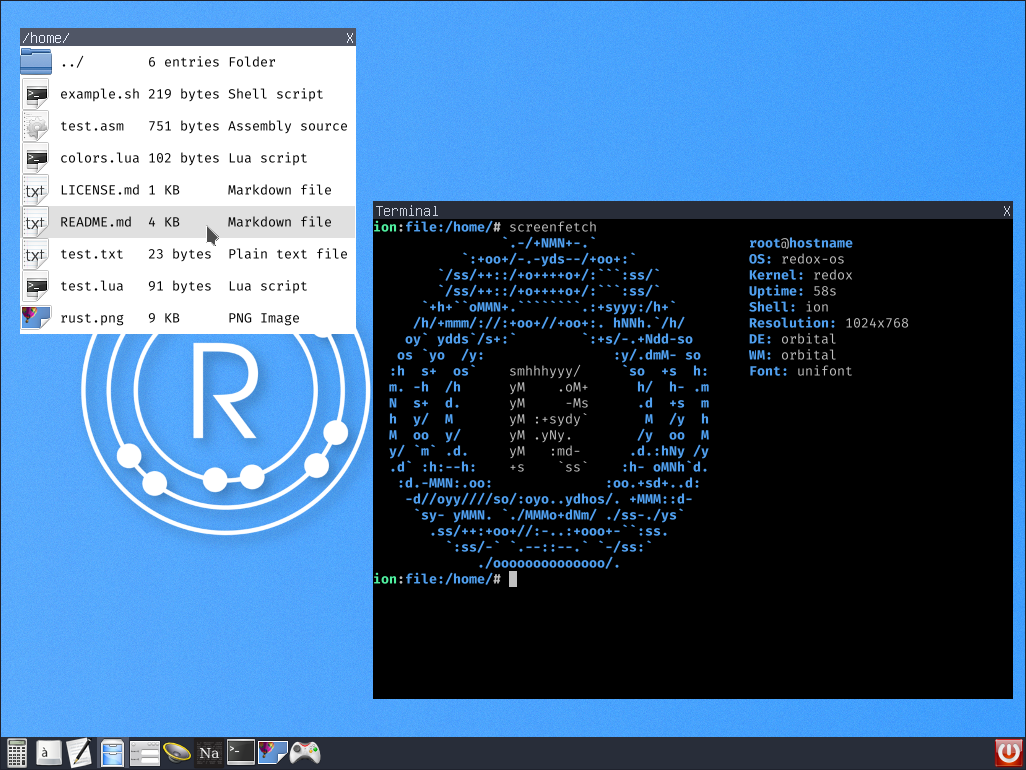
\includegraphics[width=\textwidth]{./redox.png}
        \caption{\url{https://www.redox-os.org/}}
      \end{figure}
    \end{column}
  \end{columns}
\end{frame}


\begin{frame}[c]{Blazingly Fast}
  \begin{itemize}
    \item Compiled language
    \item Uses LLVM for optimizations
    \item Zero cost abstractions
  \end{itemize}
  
\includegraphics[width=0.7\textwidth]{./spaceballs-meme.jpg}
\end{frame}


\begin{frame}[c]{Safety}
  \begin{columns}[onlytextwidth]
    \begin{column}{.3\textwidth}
      \begin{itemize}
        \item No null pointers
        \item No dangling pointers
        \item No data races
      \end{itemize}
    \end{column}
    \begin{column}{.7\textwidth}
      \begin{figure}
        
\includegraphics[width=\textwidth]{./average_cpp_programmer.png}
        \caption{Average C++ programmer}
      \end{figure}
    \end{column}
  \end{columns}
\end{frame}


\begin{frame}[c]{Ownership / Borrowing}
  \begin{itemize}
    \item Every resource has \emph{one owner}
    \item Variables are \emph{moved} to new locations
    \item Owned values can be \emph{borrowed}
      \begin{itemize}
        \item{Either: \emph{One mutable} borrow}
        \item{Or: \emph{Many immutable} borrows}
      \end{itemize}
    \item These rules are enforced by the compiler
  \end{itemize}
\end{frame}

\section{Cargo}

\begin{frame}[c]{Cargo -- Rusts Package Manager}
  \begin{columns}[onlytextwidth]
    \begin{column}{.3\textwidth}
      \centering
      \begin{figure}
      
\includegraphics[width=\textwidth]{./Cargo-Logo-Small.png}
      \end{figure}
    \end{column}
    \begin{column}{.7\textwidth}
      \begin{itemize}
        \item Awesome project and package manager
        \item Fetches and builds your project’s dependencies
        \item Invokes rustc or another build tool with the correct parameters
          to build your project
        \item packages on \url{https://crates.io} are immutable\\ $\rightarrow$
          No leftpad like disasters
      \end{itemize}
    \end{column}
  \end{columns}
\end{frame}

\section{Community}

\begin{frame}[c]{Community}
  \begin{itemize}
    \item Rust is known for its friendly and welcoming community
    \item The language is developed in the open through RFCs
    \item Active discussion on Github, Reddit, IRC, and the forum
  \end{itemize}
\end{frame}

\begin{frame}[c]{Rust in the Wild}
  Rust is already used by companies\footnote{\url{https://www.rust-lang.org/en-US/friends.html}}
  \begin{itemize}
    \item Mozilla: Servo, the Parallel Browser Engine\\
      {\footnotesize\url{https://servo.org}}
    \item Dropbox\footnote{\url{https://www.reddit.com/r/rust/comments/4adabk/the_epic_story_of_dropboxs_exodus_from_the_amazon/}}
    \item Maidsafe --- The New Decentralized Internet\\
      {\footnotesize\url{http://maidsafe.net}}
    \item Parity --- Next Generation Ethereum Client\\
      {\footnotesize\url{https://ethcore.io/parity.html}}
  \end{itemize}
\end{frame}


\section{Code Example}

\begin{frame}[c,fragile]{Code Example}
  \begin{columns}
    \begin{column}{.3\textwidth}
      \centering
      \begin{itemize}
        \item Traits based generics
        \item Pattern matching
        \item Type inference
      \end{itemize}
    \end{column}

    \begin{column}{.8\textwidth}
    \begin{minted}[fontsize=\footnotesize]{rust}
fn main() {
    let program = "+ + * - - /";
    let mut accumulator = 0;
    for token in program.chars() {
        match token {
            '+' => accumulator += 1,
            '-' => accumulator -= 1,
            '*' => accumulator *= 2,
            '/' => accumulator /= 2,
            _ => { /* ignore everything else */ }
        }
    }
    println!("The program \"{}\" calculates the value {}",
              program, accumulator);
}
  \end{minted}
      Output: \texttt{"The program "+ + * - - /" calculates the value 1"}
  \end{column}
  \end{columns}
\end{frame}


% ----------------------------------------------------------------- %

% ----------------------------------------------------------------- %

{
\setbeamertemplate{footline}{}
\pgfdeclareimage[width=\paperwidth]{bg}{background-inverted.pdf}
\usebackgroundtemplate{\pgfuseimage{bg}}
\begin{frame}[standout]
  \begin{centering}
    {\Huge Thank you!}\\
    {\normalsize \url{www.coredump.ch}}\\
  \end{centering}
\end{frame}
}

\end{document}
